% This is part of Un soupçon de mathématique sans être agressif pour autant
% Copyright (c) 2012-2014
%   Laurent Claessens
% See the file fdl-1.3.txt for copying conditions.

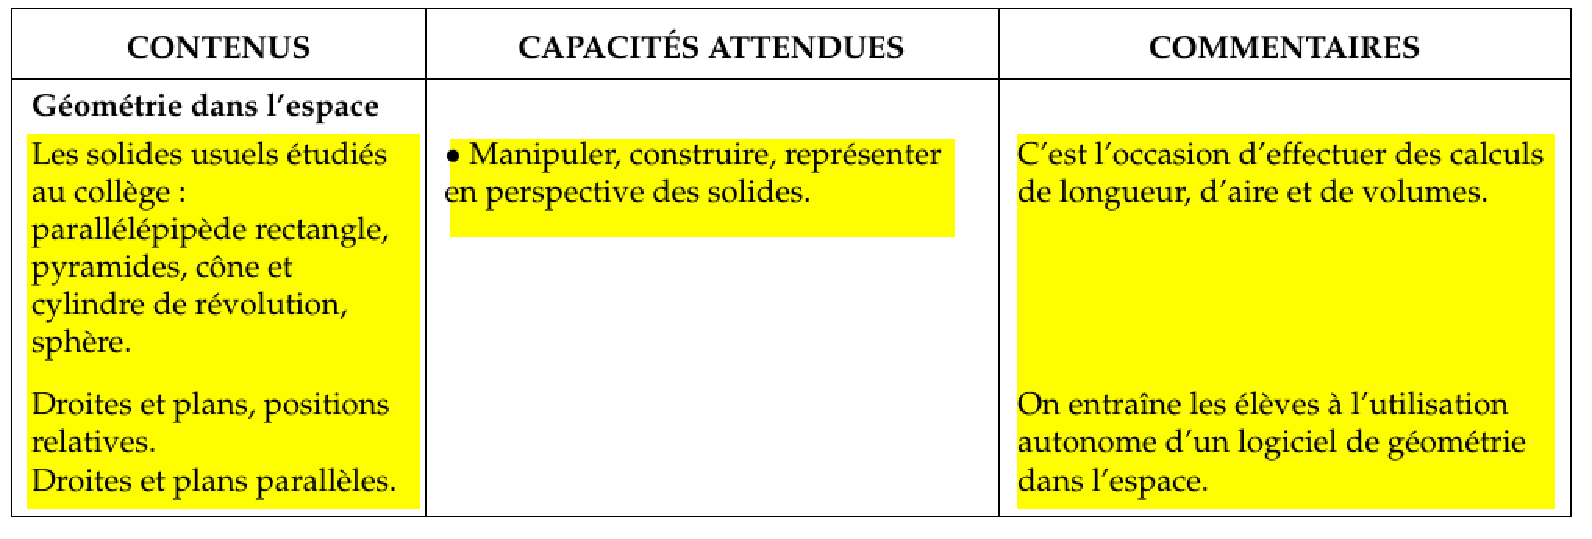
\includegraphics[width=\linewidth]{BO_perspective.pdf}

Note : La perpendiculaire n'est pas au programme. Dans ce chapitre nous allons donc nous en tenir qu'à des choses simples.

\setcounter{section}{-1}

%+++++++++++++++++++++++++++++++++++++++++++++++++++++++++++++++++++++++++++++++++++++++++++++++++++++++++++++++++++++++++++ 
\section{Activité : se poser des questions dans un cube}
%+++++++++++++++++++++++++++++++++++++++++++++++++++++++++++++++++++++++++++++++++++++++++++++++++++++++++++++++++++++++++++

% This is part of Un soupçon de mathématique sans être agressif pour autant
% Copyright (c) 2013
%   Laurent Claessens
% See the file fdl-1.3.txt for copying conditions.

\begin{wrapfigure}[3]{r}{5.0cm}
   \vspace{-0.5cm}        % à adapter.
   \centering
   \input{Fig_MEzTDZC.pstricks}
\end{wrapfigure}

À l'aide du cube ci-contre :
\begin{enumerate}
    \item
        Quelle est la nature du triangle \( AEF\) ? 
    \item
        Quelle est la nature du quadrilatère \( ABGH\) ?
    \item
        Est-ce que vous pouvez trouver trois points de ce cube formant un triangle équilatéral ?
    \item
        Si ce cube fait \unit{3}{\meter} de côté, quelle est la longueur de la «grande» diagonale \( [AG]\) ?
\end{enumerate}



Éléments de réponses :
\begin{enumerate}
    \item
        Isocèle et rectangle parce que la face supérieure est un carré.
    \item
        C'est un parallélogramme parce que il a deux côtés opposés parallèles et de même longueur : \( [AB]\) et \( [HG]\). C'est même un rectangle parce que la droite \( (AB)\) est perpendiculaire à tout le plan de la face droite (cela n'est pas précis, mais nous n'en dirons pas plus cette année).
    \item
        Il suffit de prendre trois diagonales des faces, par exemple \( AFH\).
    \item
        Effectuer Pythagore dans le triangle rectangle \( ABG\). La réponse est \( 5\sqrt{3}\) (mètres).
\end{enumerate}

%+++++++++++++++++++++++++++++++++++++++++++++++++++++++++++++++++++++++++++++++++++++++++++++++++++++++++++++++++++++++++++ 
\section{La perspective cavalière}
%+++++++++++++++++++++++++++++++++++++++++++++++++++++++++++++++++++++++++++++++++++++++++++++++++++++++++++++++++++++++++++

Le cube tracé ci-dessus est «en 3D». Il y a de nombreuses façons de dessiner en 3D, et celle que nous utilisons ici est une facile : la \defe{perspective cavalière}{perspective!cavalière}. C'est la technique la plus utilisée.

Ici : envoyer des élèves au tableau pour qu'ils montrent comment ils dessinent des cubes. On relève les éléments suivants :
\begin{enumerate}
    \item
        Les droites qui vont dans le sens de la profondeur sont dessinées en diagonale. L'angle choisit est l'\defe{angle de fuite}{angle!de fuite}.
    \item
        Elles sont dessinées un peu plus courtes. Le \defe{coefficient de réduction}{coefficient!de réduction} est le facteur «de compression» utilisé.
\end{enumerate}

Attention cependant : 
\begin{enumerate}
    \item
        Les angles et les distances ne sont pas préservées. Sur le cube plus haut, nous avons vu que le triangle \( AEF\) était rectangle et isocèle, mais sur le dessin il n'est ni l'un ni l'autre !
    \item
        Deux droites sécantes sur le dessin peuvent ne pas être sécantes dans la réalité. Par exemple \( (EH)\) et \( (AB)\).
    \item
        Un point peut paraître être sur un segment alors qu'il n'y est pas. C'est pour cela que nous avons besoin de deux yeux pour voir un 3D \ldots et donc de lunettes spéciales pour aller au cinéma en 3D.
\end{enumerate}
Pour le troisième point : montrer \emph{de visu}. D'une part en mettant un point au milieu de la face avant du cube et en disant que ça pourrait être être sur la face arrière ou même sur aucune des deux faces. Et d'autre part en montrant un bout de gomme devant une feuille. Les élèves dans l'alignement ne peuvent pas savoir si la gomme est devant ou dessus, mais les autres, oui.

Conclusion : ne pas se fier à ce que l'on voit sur le dessin.


Les avantages de cette technique sont :
\begin{propriete}
    \begin{enumerate}
        \item
             Deux segments parallèles dans la réalité sont représentés par deux segments parallèles sur le dessin.
         \item
             Trois points alignés dans la réalité sont représentés par trois points alignés sur le dessin.
         \item
             Si \( M\) est le milieu du segment \( [AB]\) dans la réalité, alors \( M\) est le milieu du segment \( [AB]\) sur le dessin.
         %\item
         %    La perspective cavalière respecte les proportions. C'est à dire que si le segment \( [AB]\) est \( p\) fois plus grand que le segment \( [CD]\) dans la réalité, alors il sera \( p\) fois plus grand sur le dessin.
    \end{enumerate}
\end{propriete}

%+++++++++++++++++++++++++++++++++++++++++++++++++++++++++++++++++++++++++++++++++++++++++++++++++++++++++++++++++++++++++++ 
\section{Ce qui est dans un plan}
%+++++++++++++++++++++++++++++++++++++++++++++++++++++++++++++++++++++++++++++++++++++++++++++++++++++++++++++++++++++++++++

Les trois suivantes permettent d'affirmer que tel point ou telle droite est dans un plan.
\begin{enumerate}
    \item
        Si \( P\) et \( Q\) sont deux points d'un plan, alors toute la droite \( (PQ)\) est encore dans ce plan.
    \item
        Si \( d\) est une droite et \( P\) est un point d'un plan, alors la parallèle à \( d\) passant par \( P\) est encore dans le plan.
    \item
        Deux droites non parallèles situées dans un même plan sont sécantes.
\end{enumerate}

%+++++++++++++++++++++++++++++++++++++++++++++++++++++++++++++++++++++++++++++++++++++++++++++++++++++++++++++++++++++++++++ 
\section{Position relatives}
%+++++++++++++++++++++++++++++++++++++++++++++++++++++++++++++++++++++++++++++++++++++++++++++++++++++++++++++++++++++++++++

%--------------------------------------------------------------------------------------------------------------------------- 
\subsection{Positions relatives de deux plans}
%---------------------------------------------------------------------------------------------------------------------------

\begin{definition}
    Deux plans sont \defe{parallèles}{parallèle!deux plans} soit si ils sont confondus, soit si ils n'ont aucun point commun. Si ils n'ont aucun point communs, nous disons qu'ils sont \defe{strictement parallèles}{parallèle!strictement}
\end{definition}

\begin{Aretenir}
    Dans les feuilles qui suivent, les deux points importants à retenir sont :
    \begin{enumerate}
        \item
            Deux plans non parallèles se coupent en une droite.
        \item
            Deux droites peuvent être ni sécantes ni parallèles.
    \end{enumerate}
\end{Aretenir}

\begin{multicols}{2}

    \begin{center}
        Plans parallèles
    \end{center}
    
\columnbreak

    \begin{center}
\input{Fig_PositionPlansTvKvah.pstricks}
    \end{center}


\end{multicols}

\begin{multicols}{2}
    \begin{center}
        Plans sécants
    \end{center}
    L'intersection de deux plans non parallèles et non confondus est une droite.

    \columnbreak

    \begin{center}
\input{Fig_PositionPlansqSltxa.pstricks}
    \end{center}

\end{multicols}

%---------------------------------------------------------------------------------------------------------------------------
\subsection{Position relative de deux droites}
%---------------------------------------------------------------------------------------------------------------------------

Deux droites peuvent être soit dans un même plan, soit ne pas être dans le même plan. Deux droites contenues dans un même plan sont dires \defe{coplanaires}{coplanaire}.

%///////////////////////////////////////////////////////////////////////////////////////////////////////////////////////////
\subsubsection{Droites coplanaires}
%///////////////////////////////////////////////////////////////////////////////////////////////////////////////////////////

Deux droites coplanaires respectent la géométrie usuelle. Elles peuvent être parallèles ou sécantes.

\vbox{
\begin{multicols}{2}
    \begin{center}
        Droites parallèles dans le plan \( (EBC)\)
    \end{center}

    \columnbreak

    \begin{center}
        \input{Fig_IDqyzXM.pstricks}
    \end{center}
\end{multicols}
}

\vbox{
\begin{multicols}{2}
    \begin{center}
        Droites sécantes dans le plan \( (AEH)\)
    \end{center}

    \columnbreak

    \begin{center}
        \input{Fig_ETfnbsh.pstricks}
    \end{center}
\end{multicols}
}

\begin{Aretenir}
    À propos de droites coplanaires :
    \begin{enumerate}
        \item
            Deux droites sécantes sont toujours coplanaires.
        \item
            Deux droites parallèles sont coplanaires.
    \end{enumerate}
\end{Aretenir}

\begin{proof}

    \begin{enumerate}
        \item

    Soient \( d\) et \( d'\) deux droites sécantes dans l'espace. Soit \( K\) leur point d'intersection; soit \( A\), un autre point sur \( d\) et \( B\) un autre point sur \( d'\).

    Le plan défini par les points \( A\), \( K\) et \( B\) contient les deux droites.

    \item

        Si \( d\) et \( d'\) sont parallèles nous considérons les points \( P\) et \( Q\) sur \( d\) et un point \( A\) sur \( d'\). D'une part droite \( d\) est dans le plan \( (PQA)\) parce que deux de ses points y sont. D'autre part la droite parallèle à \( d\) passant par \( A\) est la droite \( d'\) et est dans le plan comprenant la droite \( d\) et le point \( A\), c'est à dire le plan \( (PQA)\) également.

    \end{enumerate}
\end{proof}

%///////////////////////////////////////////////////////////////////////////////////////////////////////////////////////////
    \subsubsection{Droites non coplanaires}
%///////////////////////////////////////////////////////////////////////////////////////////////////////////////////////////
    
Deux droites non coplanaires ne peuvent pas être sécantes, ni parallèles.

\vbox{
\begin{multicols}{2}
    \begin{center}
        Il est possible pour deux droites dans l'espace d'être ni sécantes ni parallèles.
    \end{center}

    \columnbreak

    \begin{center}
        \input{Fig_ENQhxmG.pstricks}
    \end{center}
\end{multicols}
}

%---------------------------------------------------------------------------------------------------------------------------
\subsection{Position relative d'une droite et un plan}
%---------------------------------------------------------------------------------------------------------------------------

\begin{definition}
    Une droite est \defe{parallèle}{parallèle!droite et plan} à un plan lorsque soit la droite est contenue dans le plan, soit elle n'a aucun point commun avec le plan.
\end{definition}

%///////////////////////////////////////////////////////////////////////////////////////////////////////////////////////////
\subsubsection{Droite et plan sécants}
%///////////////////////////////////////////////////////////////////////////////////////////////////////////////////////////

\begin{multicols}{2}

    La droite \( (DB)\) intersecte le plan \( (AEF)\).

    \columnbreak
    \begin{center}
\input{Fig_figureBCtCTZo.pstricks}
    \end{center}
\end{multicols}

%///////////////////////////////////////////////////////////////////////////////////////////////////////////////////////////
\subsubsection{Droite et plan parallèles}
%///////////////////////////////////////////////////////////////////////////////////////////////////////////////////////////

\begin{multicols}{2}

    La droite \( (HC)\) et le plan \( (EBF)\) sont parallèles.

    \columnbreak
    \begin{center}
%The result is on figure \ref{LabelFigfigureASkECWS}. % From file figureASkECWS
%\newcommand{\CaptionFigfigureASkECWS}{<+Type your caption here+>}
\input{Fig_figureASkECWS.pstricks}
    \end{center}
\end{multicols}

%///////////////////////////////////////////////////////////////////////////////////////////////////////////////////////////
\subsubsection{Droite contenue dans un plan}
%///////////////////////////////////////////////////////////////////////////////////////////////////////////////////////////

\vbox{
\begin{multicols}{2}

    La droite \( (EB)\) est contenue dans le plan \( (AEF)\).

    \columnbreak
    \begin{center}
\input{Fig_figureCSIQETx.pstricks}
    \end{center}
\end{multicols}
}
